

% Hey
\newpage
\section{Numerical Results}%
\label{sec:numerical_results}

We want to apply the well known method of manufactured solution to solve this problem.
Let us consider the manufactured solution
\begin{equation}
    \label{eq:man_sol}
u\left( x \right) = \cos(x_{1}) \cos \left( x_{2} \right) \quad \text{ on }   \Omega =  \left( 0,2 \pi  \right)^{2}
.\end{equation}
A visualization of \eqref{eq:man_sol} can be seen on figure \ref{fig:man_sol}.
\begin{figure}[htpb]
    \centering
    \includegraphics[width=1.1\textwidth]{figures/manufactured_solution.png}
    \caption{ A illustration of the manufactured solution \eqref{eq:man_sol} on $\Omega = (0, 2 \pi ) ^2$  }
    \label{fig:man_sol}
\end{figure}
For all experiments carried out will we define $\alpha  = 1 $. We also choose the penalty parameter $ \gamma = 1$, even though the only requirement according to the results in subsection \ref{ssub:coercitivity} is that $\gamma \ge  \frac{1}{2}$. The
numerical experiments was done on the mesh discretization illustrated in figure \ref{fig:mesh_discretization}.
The FEM software package used in the implementation was gridap written in the Julia programming language \cite{verdugo22, julia17}.
On the numerical experiments shown on figures \ref{fig:man_conv},  the error norms is shown numerically that there exists a $C > 0$ such
that

On the numerical experiments shown on figures \ref{fig:man_conv},  the error norms is shown numerically that there exists a $C > 0$ such
that
\[
 \| u - u_{h} \|_{ L_{2}\left( \Omega  \right)  }^{  } \le  C  h^{p_{1}} \text{ and } \| u - h_{h} \|_{ H^{1}\left( \Omega  \right)  }  \le  C h^{p_{2}}.
\]
 We could see that for Lagrangian elements with $\mathcal{P}_{k} $ for $k = 2,3$ did the algorithm converge with $p_{1}, p_{2} \approx 2$ and for $k = 4$ was $p_{1} , p_{2} \approx 4$, which was expected.


\begin{figure}
\begin{minipage}{.4\linewidth}
\centering
\subfloat[]{\label{fig:mesh_discretization:a}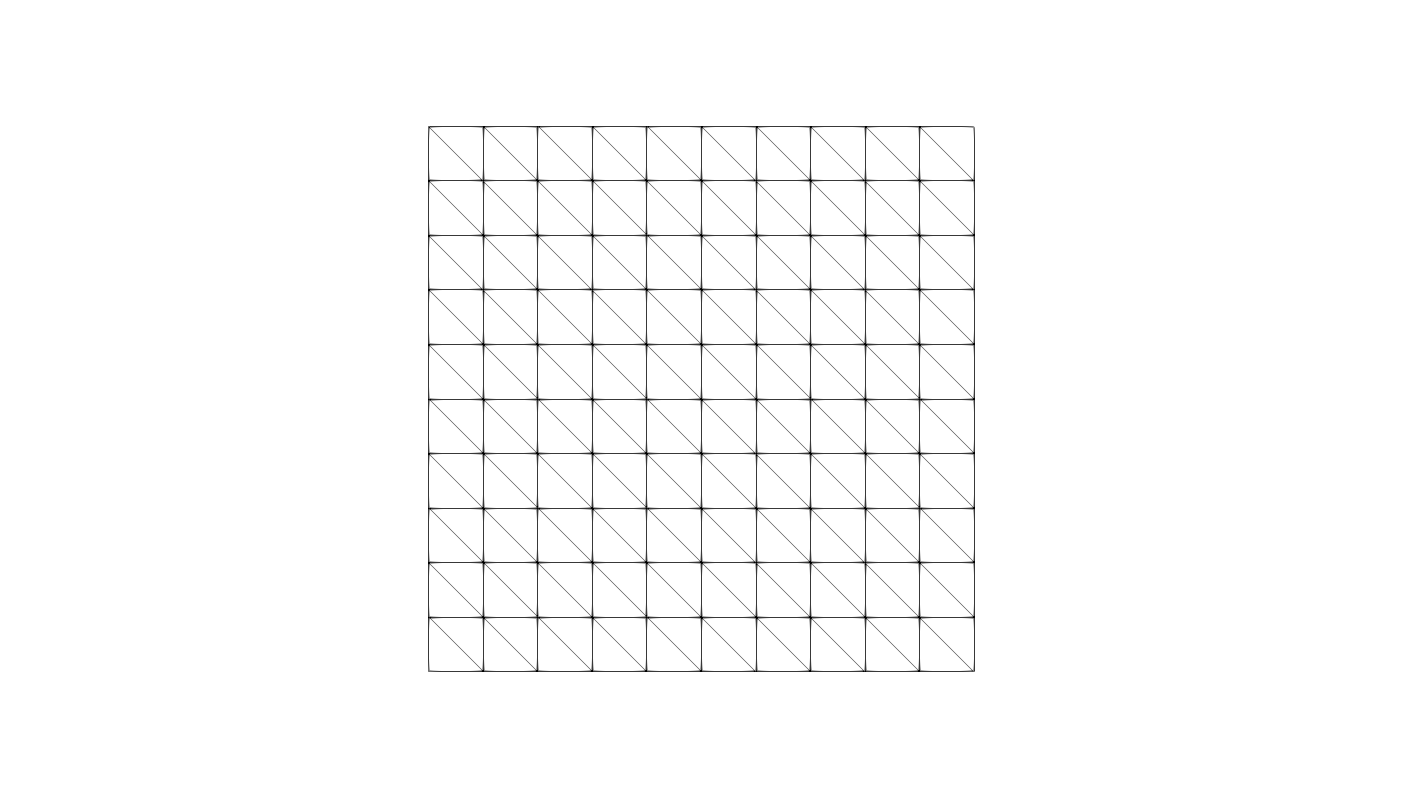
\includegraphics[scale=.15]{figures/refinements/n10.png}}
\end{minipage}%
\begin{minipage}{.4\linewidth}
\centering
\subfloat[]{\label{fig:mesh_discretization:b}\includegraphics[scale=.15]{figures/refinements/n20.png}}
\end{minipage}\par\medskip
\centering
\subfloat[]{\label{fig:mesh_discretization:c}\includegraphics[scale=.15]{figures/refinements/n40.png}}

\caption{Illustration of mesh discretization on the unit square $\Omega = (0,2 \pi)^{2} \subseteq  \mathbb{R} ^{2}$
    with triangulation $\mathcal{T} _{h}$. The chosen instances had the diameters $h = \left\{ 2\pi  /10, 2\pi /20,2\pi /40 \right\}$ in figures \ref{fig:mesh_discretization:a},
    \ref{fig:mesh_discretization:b} and \ref{fig:mesh_discretization:c}.
}

\label{fig:mesh_discretization}
\end{figure}


\begin{figure}
    \centering
\begin{minipage}{.5\linewidth}
\centering
\subfloat[]{\label{fig:man_conv:a}\includegraphics[scale=.05]{figures/convergence/convergence_d_2.png}}
\end{minipage}%
\begin{minipage}{.5\linewidth}
\centering
\subfloat[]{\label{fig:man_conv:b}\includegraphics[scale=.05]{figures/convergence/convergence_d_3.png}}
\end{minipage}\par\medskip
\centering
\subfloat[]{\label{fig:man_conv:c}\includegraphics[scale=.05]{figures/convergence/convergence_d_4.png}}


\caption{ Convergence plots for $\| u - u_{h} \|_{ L_{2}\left( \Omega  \right)  }^{  } \le Ch^{p_{1}} $ and $\| u - u_{h} \|_{ H^{1}\left( \Omega  \right)   }^{  }\le Ch^{p_{2}} $  using Lagrangian elements with polynomials $\mathcal{P}_{k} $ with
    order $k$ .
    Figures \ref{fig:man_conv:a},
\ref{fig:man_conv:b} and \ref{fig:man_conv:c} has respectively the order $k=2,3, 4$.  }
\label{fig:man_conv}
\end{figure}


% \begin{figure}
% \begin{center}
% \begin{tabular}{|c|c|}
% \toprule

% \textbf{A} & \adjustimage{height=8cm,valign=m}{PlotA} \\
% \midrule
% \textbf{B} & \adjustimage{height=8cm,valign=m}{PlotB} \\
% \midrule
% \textbf{C} & \adjustimage{height=8cm,valign=m}{PlotC} \\

% \bottomrule
% \end{tabular}
% \end{center}
% \caption{I don't want a table: Andrew Cashner's way} \label{faketable:mul}

% \end{figure}

\begin{table}
  \begin{tabular}{rrrrr}
    \hline\hline
    \textbf{h} & \textbf{$L_2$} & \textbf{$H^1$} & \textbf{$log_2(e^{2h}_{L^2(\Omega )}/e^{h}_{L^2(\Omega )}) $} & \textbf{$log_2(e^{2h}_{H_1(\Omega )}/e^{h}_{H_1(\Omega )}) $} \\\hline
    7.854E-01 & 9.380E+00 & 2.269E+00 &  &  \\
    3.927E-01 & 4.891E-01 & 1.410E-01 & -2.954E+00 & -2.778E+00 \\
    1.963E-01 & 1.180E-01 & 3.939E-02 & -1.422E+00 & -1.276E+00 \\
    9.817E-02 & 3.695E-02 & 1.107E-02 & -1.161E+00 & -1.269E+00 \\\hline\hline
  \end{tabular}
\end{table}


